\documentclass[a4paper,12pt]{report}
\usepackage[utf8]{inputenc}
\usepackage[T1]{fontenc}
\usepackage[english, indonesian]{babel}
\usepackage{times}
\usepackage{graphicx}
\usepackage{setspace}
\usepackage{titlesec}
\usepackage{fancyhdr}
\usepackage{enumitem}
\usepackage{amsmath, amssymb}
\usepackage{hyperref}
\usepackage{booktabs}
\usepackage{tabularx}
\usepackage[section]{placeins}  % FloatBarrier sebelum tiap section, agar tabel/gambar tidak terselip

\usepackage{indentfirst}

\usepackage[left=2.5cm, right=2.5cm, top=2.5cm, bottom=2.5cm]{geometry}

\titleformat{\chapter}[display]
  {\normalfont\Large\bfseries\centering}{\MakeUppercase{\chaptername} \thechapter}{15pt}{\Large}
\titlespacing*{\chapter}{0pt}{-25pt}{20pt}

\titleformat{\section}
  {\normalfont\large\bfseries}{\thesection}{1em}{}
\titlespacing*{\section}{0pt}{10pt}{10pt}

\titleformat{\subsection}
  {\normalfont\normalsize\bfseries}{\thesubsection}{1em}{}
\titlespacing*{\subsection}{1.5em}{8pt}{6pt}

\setlength{\parindent}{1.25em}
\setlength{\parskip}{0pt}

\pagestyle{fancy}
\fancyhf{}
\fancyfoot[C]{\small\thepage}
\renewcommand{\headrulewidth}{0pt}
\renewcommand{\footrulewidth}{0.4pt}

\fancypagestyle{plain}{
  \fancyhf{}
  \fancyfoot[C]{\small\thepage}
  \renewcommand{\headrulewidth}{0pt}
  \renewcommand{\footrulewidth}{0.4pt}
}

\onehalfspacing

% Jarak antar baris tabel agar lebih lega
\renewcommand{\arraystretch}{1.4}

\begin{document}

\begin{titlepage}
    \centering
    \vspace*{1cm}
    
    {\normalsize\bfseries Progress Project SDA \par}
    {\normalsize\bfseries Pengembangan Aplikasi Web Interaktif untuk Visualisasi Graf Molekul \par}
    {\normalsize\bfseries dan Eksplorasi Properti Kuantum pada Dataset QM9 \par}
    
    \vspace{2cm}
    
    
\includegraphics[width=0.40\textwidth]{logo_unesa.png}
    
    \vspace{1.8cm}
    
    {\normalsize\bfseries DOSEN PENGAMPU: \par}
    {\normalsize Yuni Rosita Dewi, M.Si. \par}
    
    \vspace{1.5cm}
    
    {\normalsize\bfseries DISUSUN OLEH: \par}
    \vspace{0.7cm}
    \begin{tabular}{ll}
        M. Habiburrohman Al-Fathir          & (24031554145) \\
        Arzha Dwi Ananda Anhar Wijaya       & (25031554264) \\
        Muhammad Pasha Paksi Pasukopati     & (25031554019)
    \end{tabular}
    
    \vfill
    
    {\normalsize PROGRAM STUDI S1 SAINS DATA \par}
    {\normalsize FAKULTAS MATEMATIKA DAN ILMU PENGETAHUAN ALAM \par}
    {\normalsize UNIVERSITAS NEGERI SURABAYA \par}
    {\normalsize 2026 \par}
    
\end{titlepage}

\tableofcontents
\newpage

\chapter{PENDAHULUAN}

\section{Latar Belakang}

Graf adalah salah satu contoh struktur data dasar dalam ilmu komputer yang digunakan untuk merepresentasikan hubungan elemen melalui himpunan titik yang disebut \textit{node} (atau verteks) dan garis penghubung yang disebut \textit{edge} (atau sisi). Dalam bidang kimia komputasional, molekul secara alami dapat divisualisasikan sebagai graf, di mana atom berperan sebagai \textit{node} dan ikatan kimia berperan sebagai \textit{edge}. Representasi ini menjadi dasar bagi berbagai pendekatan \textit{graph-based learning}, termasuk yang didemonstrasikan dalam paper \textit{``Adaptive edge-aware graph convolutional with multi-task learning for simultaneous prediction of material properties''} yang menggunakan \textit{graph neural network} pada dataset QM9.

Dataset QM9 berisi sekitar 133 ribu molekul organik kecil dengan koordinat 3D dan 16 properti kuantum. Namun, informasi ikatan (\textit{edge}) tidak disediakan secara eksplisit, hanya koordinat atom yang tersedia. Hal ini menimbulkan tantangan menarik dari perspektif mata kuliah Struktur Data dan Algoritma yaitu bagaimana membangun graf dari data spasial? Bagaimana menyimpan dan menampilkan graf tersebut secara efisien?

Proyek ini mengembangkan aplikasi web interaktif yang menerapkan konsep-konsep utama Struktur Data dan Algoritma, yaitu struktur graf, algoritma pembangunan graf, algoritma penataan tata letak graf, dan strategi penyimpanan sementara (\textit{caching}), untuk memproses dan menampilkan molekul-molekul QM9 dalam bentuk graf dua dimensi.

\section{Rumusan Masalah}
\begin{enumerate}[label=\arabic*.]
    \item Bagaimana membangun graf molekul (pembuatan \textit{edge}) dari koordinat 3D atom menggunakan algoritma berbasis jarak?
    \item Bagaimana menyimpan graf molekul dengan efisien ke dalam memori (\textit{adjacency list} dibandingkan dengan \textit{adjacency matrix}) untuk mendukung operasi traversal dan visualisasi?
    \item Bagaimana menghitung tata letak dua dimensi graf menggunakan algoritma \textit{force-directed} (Kamada-Kawai dan Fruchterman-Reingold) sehingga struktur molekul terlihat jelas?
    \item Bagaimana menerapkan struktur data \textit{hash map} (\textit{dictionary}) untuk pencarian cepat dan penyimpanan sementara (\textit{caching}) untuk menghindari perhitungan berulang?
    \item Bagaimana membangun antarmuka web interaktif yang memungkinkan eksplorasi dan perbandingan graf molekul?
\end{enumerate}

\section{Tujuan}
\begin{enumerate}[label=\arabic*.]
    \item Mengimplementasikan algoritma pembangunan graf dari data spasial, yaitu koordinat 3D diubah menjadi \textit{edge} berdasarkan jarak kovalen.
    \item Mengimplementasikan representasi graf menggunakan \textit{adjacency list} (melalui \textit{library} NetworkX) dan \textit{hash map} untuk pengindeksan.
    \item Mengimplementasikan algoritma tata letak dua dimensi \textit{force-directed}, yaitu Kamada-Kawai dengan alternatif Fruchterman-Reingold.
    \item Menerapkan strategi penyimpanan sementara (\textit{caching}), yaitu penulisan ke format \textit{pickle} dan JSON, untuk efisiensi pengolahan data.
    \item Membangun aplikasi web monolitik (menggunakan FastAPI, JavaScript murni, dan Cytoscape.js) untuk visualisasi interaktif.
\end{enumerate}

\section{Manfaat}
\begin{itemize}
    \item \textbf{Akademik}: Mendemonstrasikan penerapan struktur data graf, \textit{hash map}, dan algoritma penataan graf pada data dunia nyata.
    \item \textbf{Praktis}: Memudahkan eksplorasi struktur dan properti molekul QM9 tanpa menulis kode.
    \item \textbf{Edukatif}: Menjadi media pembelajaran interaktif untuk memahami hubungan antara representasi graf dan sifat-sifat molekul.
\end{itemize}

\section{Batasan}
\begin{enumerate}[label=\arabic*.]
    \item Dataset diakses penuh (133.885 molekul) lewat \textit{index hash map}. Detail molekul (graf, koordinat) dibaca dari file \texttt{.xyz} hanya saat dibutuhkan (\textit{lazy load}).
    \item Pembentukan \textit{edge} menggunakan pendekatan berbasis jarak (jari-jari kovalen ditambah toleransi), bukan dari data topologi eksplisit, sehingga tidak membedakan ikatan tunggal, ganda, maupun tiga.
    \item Visualisasi hanya dalam bentuk graf dua dimensi, tidak ada tampilan struktur tiga dimensi.
    \item Algoritma tata letak menggunakan pustaka NetworkX, tidak dibangun dari dasar.
\end{enumerate}

\chapter{TINJAUAN PUSTAKA}

\section{Struktur Data Graf}

Graf $G = (V, E)$ adalah suatu struktur data yang terdiri dari himpunan \textit{node} (verteks) $V$ dan himpunan \textit{edge} (sisi) $E$. Terdapat dua cara utama untuk menyimpan graf dalam memori komputer, yaitu \textit{adjacency matrix} dan \textit{adjacency list}.

\subsection{Adjacency Matrix}

\textit{Adjacency matrix} adalah matriks berukuran $n \times n$ di mana entri ke-$i$ dan ke-$j$ bernilai 1 jika terdapat \textit{edge} dari \textit{node} $i$ ke \textit{node} $j$, dan 0 jika tidak.

\begin{itemize}
    \item \textbf{Kelebihan}: Pengecekan adanya \textit{edge} sangat cepat, yaitu $O(1)$, sehingga cocok untuk graf yang padat (\textit{dense}).
    \item \textbf{Kekurangan}: Membutuhkan memori $O(n^2)$, sehingga tidak efisien untuk graf yang memiliki sedikit \textit{edge} (graf \textit{sparse}).
\end{itemize}

\subsection{Adjacency List}

\textit{Adjacency list} adalah struktur di mana setiap \textit{node} menyimpan daftar \textit{node} tetangganya. Dalam implementasi Python, ini direpresentasikan sebagai \textit{dictionary} yang berisi \textit{list} tetangga.

\begin{itemize}
    \item \textbf{Kelebihan}: Konsumsi memori $O(V + E)$, sehingga sangat efisien untuk graf yang memiliki sedikit \textit{edge} (graf \textit{sparse}) seperti graf molekul.
    \item \textbf{Kekurangan}: Pengecekan \textit{edge} memerlukan $O(\text{degree})$, tidak secepat matriks.
\end{itemize}

Graf molekul bersifat \textbf{sparse}, artinya molekul dengan $n$ atom memiliki maksimal $n-1$ ikatan (untuk graf yang terhubung), jumlah yang jauh lebih kecil dari $n^2$ kemungkinan \textit{edge}. Oleh sebab itu, \textbf{\textit{adjacency list}} merupakan representasi yang lebih tepat.

\section{Pembentukan Graf dari Data Spasial}

Dalam dataset QM9, informasi \textit{edge} (ikatan) tidak tersedia secara eksplisit. Graf harus dibangun dengan algoritma berbasis jarak. Dua atom $i$ dan $j$ dianggap berikatan jika jarak Euclidean antar-keduanya kurang dari jumlah jari-jari kovalen ditambah nilai toleransi. Secara matematis:

\[
d_{ij} < r_i^{\text{cov}} + r_j^{\text{cov}} + \delta
\]

Di mana $d_{ij} = \sqrt{(x_i - x_j)^2 + (y_i - y_j)^2 + (z_i - z_j)^2}$ adalah jarak Euclidean antara atom $i$ dan $j$, $r_i^{\text{cov}}$ adalah jari-jari kovalen atom $i$, dan $\delta = 0{,}45$ \r{A} adalah toleransi yang ditambahkan untuk mengakomodasi variasi dalam data.

Algoritma ini memeriksa semua pasangan atom, sehingga memiliki kompleksitas \textbf{$O(n^2)$}. Untuk molekul QM9 yang memiliki paling banyak 29 atom, kompleksitas ini masih sangat efisien. Untuk dataset yang lebih besar, dapat dioptimasi menggunakan teknik \textit{spatial indexing} (seperti kd-tree) menjadi $O(n \log n)$.

\section{Algoritma Tata Letak Graf Dua Dimensi}

Tata letak graf (\textit{layout}) adalah suatu proses yang dilakukan untuk menentukan posisi \textit{node} pada bidang dua dimensi agar graf dapat divisualisasikan dengan jelas. Dua algoritma \textit{force-directed} yang digunakan adalah Kamada-Kawai dan Fruchterman-Reingold.

\subsection{Kamada-Kawai}

Algoritma ini memodelkan graf sebagai sistem pegas, di mana setiap pasangan \textit{node} dihubungkan oleh pegas yang memiliki panjang ideal. Panjang ideal tersebut sebanding dengan jarak terpendek (\textit{shortest path}) antara kedua \textit{node} dalam graf. Energi total sistem dirumuskan sebagai:

\[
E = \sum_{i<j} k_{ij} \left( |p_i - p_j| - l_{ij} \right)^2
\]

Di mana $k_{ij}$ adalah konstanta pegas dan $l_{ij}$ adalah panjang ideal. Posisi \textit{node} dioptimasi menggunakan metode Newton-Raphson hingga sistem mencapai keadaan stabil (konvergen).

\begin{itemize}
    \item \textbf{Kompleksitas}: $O(n^2)$ per iterasi, dan $O(n^3)$ untuk perhitungan jarak terpendek awal.
    \item \textbf{Kelebihan}: Menghasilkan tata letak yang terstruktur dan mudah dibaca.
    \item \textbf{Kekurangan}: Lambat untuk graf besar; tidak dapat menangani graf yang terpisah menjadi beberapa bagian (tidak terhubung).
\end{itemize}

\subsection{Fruchterman-Reingold (Spring Layout)}

Algoritma ini mensimulasikan gaya tarik antara \textit{node} yang bertetangga dan gaya tolak antara semua \textit{node} secara berulang. Gaya tarik sebesar $d^2/k$ menarik \textit{node} yang berikatan, sedangkan gaya tolak sebesar $-k^2/d$ menolak semua \textit{node}, dengan $k$ adalah konstanta dan $d$ adalah jarak aktual. Posisi diperbarui setiap iterasi dengan jadwal pendinginan sementara (\textit{cooldown}).

\begin{itemize}
    \item \textbf{Kompleksitas}: $O(n^2)$ per iterasi karena menghitung gaya tolak untuk setiap pasangan \textit{node}.
    \item \textbf{Kelebihan}: Dapat menangani graf yang tidak terhubung.
    \item \textbf{Kekurangan}: Tata letak yang dihasilkan kurang terstruktur dibandingkan Kamada-Kawai.
\end{itemize}

\section{Struktur Data Pendukung}

\subsection{Hash Map (Dictionary)}

\textit{Hash map}, yang dalam Python disebut \textit{dictionary} atau \textit{dict}, adalah struktur data yang memungkinkan pencarian nilai berdasarkan kunci dengan kompleksitas $O(1)$. Dalam proyek ini, \textit{hash map} digunakan untuk beberapa keperluan:
\begin{itemize}
    \item Pemetaan ID molekul ke posisi dalam \textit{array} untuk pencarian cepat berdasarkan ID.
    \item Pemetaan SMILES ke nama molekul yang diperoleh dari \textit{PubChem API}.
    \item Pemetaan elemen kimia ke jari-jari kovalen untuk pembentukan ikatan.
    \item Pemetaan elemen kimia ke warna untuk visualisasi \textit{node}.
\end{itemize}

\subsection{Array (NumPy ndarray)}

\textit{Array} (dalam bentuk \textit{NumPy ndarray}) digunakan untuk menyimpan koordinat 3D atom secara berurutan ke dalam memori. Hal ini memungkinkan operasi matematika (seperti perhitungan jarak Euclidean) dilakukan secara efisien melalui teknik \textit{vectorisasi}.

\subsection{Serialization (Pickle dan JSON)}

\textit{Serialization} adalah proses mengubah objek data menjadi bentuk yang dapat disimpan ke file. \textit{Pickle} digunakan untuk menyimpan dataset dalam format biner Python, yang cepat dan mendukung objek kompleks. JSON digunakan untuk menyimpan cache nama molekul dalam format teks, yang mudah dibaca manusia dan dapat digunakan oleh berbagai bahasa pemrograman lainnya.

\section{Dataset QM9}

Dataset QM9 dipilah oleh Ramakrishnan et al.\ (2014) dan dipublikasikan dalam jurnal \textit{Scientific Data}. Dataset ini merupakan bagian dari GDB-17, yaitu \textit{database} virtual yang memuat sekitar 166 miliar molekul organik kecil. QM9 memilih molekul yang memiliki paling banyak 9 atom berat (karbon, nitrogen, oksigen, fluor) dan menghitung properti kuantumnya menggunakan metode DFT pada level B3LYP/6-31G(2df,2p).

Setiap molekul dalam file \texttt{.xyz} memuat: jumlah atom, 16 properti kuantum, koordinat 3D setiap atom, frekuensi vibrasi, string SMILES, dan kode InChI.

\section{Teknologi yang Digunakan}

Berikut adalah teknologi yang digunakan dalam pengembangan aplikasi beserta perannya dalam konteks Struktur Data dan Algoritma.

\begin{table}[htbp]
\centering
\small
\begin{tabularx}{\textwidth}{l l X}
\toprule
\textbf{Komponen} & \textbf{Teknologi} & \textbf{Peran dalam SDA} \\
\midrule
\textit{Backend}   & Python 3 + FastAPI       & Menyediakan API dan pengolahan data graf \\
\textit{Library} Graf      & NetworkX                 & Representasi graf dan algoritma tata letak \\
Komputasi Numerik   & NumPy                    & Operasi \textit{array} dan perhitungan jarak \\
Penyimpanan & Pickle, JSON           & Penyimpanan data hasil komputasi \\
\textit{Frontend}  & JavaScript + Cytoscape.js & Tampilan graf interaktif di peramban \\
\bottomrule
\end{tabularx}
\end{table}

\chapter{METODOLOGI}

\section{Arsitektur Sistem}

Sistem dikembangkan dengan arsitektur \textbf{monolitik}, artinya satu perangkat lunak \textit{server} (menggunakan FastAPI) menangani semua permintaan baik data maupun berkas statis. Pendekatan ini dipilih untuk menghindari kerumitan komunikasi antar-bagian dan memfokuskan implementasi pada pengelolaan struktur data graf.

Pada sisi klien, peramban web (\textit{browser}) menjalankan Cytoscape.js dari CDN untuk menampilkan graf (\textit{node} dan \textit{edge}) serta mengirim permintaan HTTP ke \textit{server}. Pada sisi \textit{server}, FastAPI menyediakan API (GET /molecules, GET /mol/\{id\}, POST /compare) dan berkas statis (index.html, style.css, app.js). Di balik komunikasi ini, ada komponen Struktur Data dan Algoritma mengelola \textit{hash map} untuk pencarian molekul dengan kompleksitas $O(1)$, graf NetworkX dengan \textit{adjacency list}, \textit{array} NumPy untuk koordinat, serta penyimpanan sementara dalam format Pickle untuk data dan JSON untuk nama.

\section{Algoritma Pembentukan Graf}

\subsection{Pengolahan Data Mentah}

File \texttt{.xyz} dibaca baris per baris. Data diekstrak ke dalam beberapa struktur: daftar elemen atom (\textit{atoms}) yang berfungsi sebagai ID \textit{node}, matriks koordinat 3D berukuran $n \times 3$ (\textit{coords}) dalam bentuk \textit{array} NumPy, \textit{hash map} properti kuantum, dan string SMILES untuk pencarian nama.

\subsection{Pembentukan Edge (Inferensi Ikatan)}

Algoritma inferensi ikatan bekerja secara \textit{pairwise}, artinya memeriksa semua kombinasi pasangan atom satu per satu. Untuk setiap pasangan atom $i$ dan $j$ (hanya bagian segitiga atas karena graf tidak berarah), algoritma melakukan pencarian jari-jari kovalen masing-masing atom dari \textit{hash map} COVALENT\_RADII (kompleksitas $O(1)$), menghitung jarak Euclidean antar-koordinat, lalu membandingkan dengan jumlah jari-jari kovalen ditambah toleransi. Jika jarak kurang dari ambang batas, pasangan tersebut ditambahkan ke daftar \textit{edge}.

\textbf{Kompleksitas}: Waktu $O(n^2)$ dan ruang $O(E)$, yang cukup efisien untuk graf molekul yang berukuran kecil.

\subsection{Pembentukan Objek Graf}

Daftar \textit{edge} hasil inferensi diubah menjadi objek graf NetworkX yang menggunakan \textit{adjacency list} secara internal. Setiap \textit{node} ditambahkan dengan atribut elemen kimia terkain, dan setiap \textit{edge} ditambahkan dengan bobot berupa jarak antar-atom.

\section{Algoritma Tata Letak Dua Dimensi}

Algoritma tata letak menciptakan graf dari data atom dan ikatan terlebih dahulu. Jika graf hanya memiliki satu \textit{node}, posisi dikembalikan di titik awal (origin). Untuk graf yang lebih besar, algoritma mencoba Kamada-Kawai terlebih dahulu karena menghasilkan tata letak yang terstruktur. Jika gagal (misalnya graf terpisah menjadi beberapa bagian), digunakan Fruchterman-Reingold sebagai alternatif. Setelah tata letak diperoleh, posisi dinormalisasi ke rentang $\pm$150 piksel dan dipusatkan pada titik origin.

\section{Strategi Penyimpanan Sementara (Caching) dan Indeks}

Memproses ulang 133.885 file \texttt{.xyz} setiap kali aplikasi dijalankan jelas tidak efisien. Karena itu, sistem menggunakan tiga tingkat penyimpanan:

\begin{table}[htbp]
\centering
\small
\begin{tabularx}{\textwidth}{c l l X}
\toprule
\textbf{Tingkat} & \textbf{Struktur Data} & \textbf{Format} & \textbf{Isi} \\
\midrule
1 & \textit{Hash map} indeks  & JSON   & Metadata semua molekul: formula, SMILES, nama, 16 properti kuantum \\
2 & \textit{Hash map} cache   & Pickle & Detail molekul yang sudah pernah dibuka (graf + tata letak 2D) \\
3 & \textit{Hash map} nama   & JSON   & Cache SMILES ke nama dari PubChem \\
\bottomrule
\end{tabularx}
\end{table}

Saat aplikasi dijalankan pertama kali, skrip \texttt{setup.py} membangun indeks dengan memindai 133.885 file \texttt{.xyz} dan mengekstrak metadata. Hasilnya disimpan ke \texttt{index.json}. Pemindaian ini hanya dilakukan sekali; pada peluncuran berikutnya, indeks langsung dimuat dari \textit{disk} dalam waktu kurang dari satu detik.

Saat pengguna membuka detail molekul, sistem memeriksa cache \texttt{.pkl} terlebih dahulu. Jika tersedia, data dikembalikan dengan kompleksitas $O(1)$. Jika tidak, file \texttt{.xyz} terkait dibaca, ikatan disimpulkan, tata letak 2D dihitung, lalu hasilnya disimpan ke cache supaya akses berikutnya instan. Pendekatan \textit{lazy load} ini menghindari pemrosesan dini terhadap data yang belum tentu dibutuhkan.

\section{Operasi Query pada Dataset}

Berikut adalah daftar operasi query yang tersedia pada dataset beserta struktur data dan kompleksitas masing-masing.

\begin{table}[htbp]
\centering
\small
\begin{tabularx}{\textwidth}{X l c}
\toprule
\textbf{Operasi} & \textbf{Struktur Data} & \textbf{Kompleksitas} \\
\midrule
Menampilkan daftar molekul      & \textit{Array} (potongan)          & $O(\text{limit})$ \\
Mencari molekul berdasarkan ID   & \textit{Hash map} \texttt{meta} & $O(1)$ \\
Mencari berdasarkan rumus kimia  & \textit{Hash map} \texttt{formula\_idx} & $O(1)$ \\
Mencari berdasarkan SMILES       & \textit{Hash map} \texttt{smiles\_idx}  & $O(1)$ \\
Mencari berdasarkan nama (substring) & Pencarian berurutan            & $O(n)$ \\
Membandingkan molekul            & \textit{Hash map} sebanyak $k$    & $O(k)$ \\
Menghitung statistik properti     & Penggabungan \textit{array}       & $O(n)$ per properti \\
Membentuk graf dari notasi (\textit{fallback})  & Parser SMILES + Kamada-Kawai & $O(n^3)$ \\
\bottomrule
\end{tabularx}
\end{table}

\chapter{IMPLEMENTASI}

\section{Struktur Proyek}

Proyek disusun dalam satu direktori \textit{root} yang berisi berkas README.md, setup.py (skrip otomatisasi unduh dan instalasi), report (LaTeX), dan .gitignore. Direktori \textit{backend} memuat main.py sebagai aplikasi FastAPI, qm9\_loader.py untuk membaca berkas .xyz dan mencari nama dari PubChem, graph\_processor.py untuk membentuk graf dan menghitung tata letak dua dimensi, data\_manager.py untuk \textit{lazy load} molekul dan pengelolaan cache, index\_builder.py untuk memindai semua \texttt{.xyz} dan membangun \textit{hash map} indeks, smiles\_parser.py untuk membentuk graf dari notasi SMILES (\textit{fallback} ketika molekul tidak ada di dataset), serta requirements.txt. Subdirektori static memuat index.html, style.css, dan app.js. Direktori data memuat qm9\_raw untuk berkas .xyz asli dan qm9\_processed untuk index.json, cache.pkl, dan names\_cache.json.

\section{Implementasi Struktur Data Graf}

\subsection{Pembentukan Edge pada graph\_processor.py}

Fungsi infer\_bonds menerapkan algoritma \textit{pairwise} untuk mendeteksi ikatan. Konstanta jari-jari kovalen disimpan dalam \textit{hash map} COVALENT\_RADII. Fungsi mengiterasi semua pasangan atom menggunakan dua \textit{nested loops} (hanya bagian segitiga atas karena graf tidak berarah). Untuk setiap pasangan, jari-jari kovalen diambil dari \textit{hash map} (kompleksitas $O(1)$), jarak Euclidean dihitung menggunakan NumPy, dan jika jarak kurang dari jumlah jari-jari kovalen ditambah toleransi, \textit{edge} ditambahkan ke daftar.

Analisis kompleksitas: waktu $O(n^2)$ karena memeriksa semua pasangan, dan ruang $O(E)$ untuk daftar \textit{edge}, dengan $E \leq n(n-1)/2$ namun pada praktiknya $E \approx n$ karena graf molekul bersifat \textit{sparse}.

\subsection{Pembangunan Graf pada graph\_processor.py}

Fungsi compute\_2d\_layout membuat objek NetworkX Graph yang menggunakan \textit{adjacency list}. \textit{Node} ditambahkan dengan atribut elemen, dan \textit{edge} ditambahkan dengan bobot jarak. Jika graf hanya memiliki satu atom, posisi diletakkan di origin. Jika lebih besar, algoritma mencoba Kamada-Kawai. Jika gagal (misalnya graf terpisah), digunakan Fruchterman-Reingold sebagai alternatif. Posisi kemudian dinormalisasi ke rentang $\pm$150 piksel.

Analisis kompleksitas: Kamada-Kawai membutuhkan $O(n^3)$ untuk perhitungan jarak terpendek awal (algoritma Floyd-Warshall) dan $O(n^2)$ per iterasi Newton-Raphson. Fruchterman-Reingold membutuhkan $O(n^2)$ per iterasi karena menghitung gaya tolak untuk setiap pasangan, sehingga total $O(\text{iterasi} \times n^2)$.

\subsection{Hash Map untuk Pengindeksan pada data\_manager.py}

Kelas QM9Dataset menggunakan beberapa \textit{hash map} sekaligus untuk mendukung pencarian cepat. Pertama, \texttt{meta} memetakan \texttt{mol\_id} ke metadata molekul (formula, SMILES, nama, properti) untuk akses $O(1)$ berdasarkan ID. Kedua, \texttt{formula\_idx} memetakan rumus kimia (notasi Hill, misalnya \texttt{C6H6}) ke daftar \texttt{mol\_id} yang memiliki rumus tersebut. Ketiga, \texttt{smiles\_idx} memetakan string SMILES ke \texttt{mol\_id} (asumsi unik dalam QM9).

Metode \texttt{get\_molecule} memeriksa cache \textit{pickle} terlebih dahulu. Jika tidak ada, file \texttt{.xyz} dibaca, ikatan disimpulkan, tata letak dihitung, lalu hasilnya disimpan ke cache. Akses berikutnya untuk molekul yang sama jadi $O(1)$.

Rantai pencarian berdasarkan rumus kimia: rumus ke \textit{hash map} \texttt{formula\_idx} ke daftar ID ke \textit{hash map} \texttt{meta}. Total kompleksitas: \textbf{$O(1)$}.

\subsection{Penyimpanan Sementara pada data\_manager.py}

Cache \textit{pickle} berbentuk \textit{hash map} \texttt{mol\_id ke molekul lengkap} (graf, koordinat, tata letak 2D, properti). Cache ini bertambah secara bertahap: hanya molekul yang pernah dibuka pengguna yang masuk. Setiap kali ada molekul baru ditambahkan, seluruh cache di-\textit{flush} kembali ke \textit{disk}. Operasi pemuatan dan penyimpanan masing-masing $O(n)$ terhadap jumlah molekul yang sudah di-cache.

\subsection{Pencarian Nama Molekul pada qm9\_loader.py}

Nama molekul dicari melalui dua tahap. Pertama, menggunakan \textit{dictionary} lokal SMILES\_TO\_NAME yang berisi sekitar 50 SMILES umum. Kedua, untuk SMILES yang tidak ada di \textit{dictionary}, dilakukan permintaan ke \textit{PubChem PUG REST API}. Hasil pencarian disimpan permanen ke berkas names\_cache.json dalam format \textit{hash map} (SMILES ke nama), sehingga API hanya dipanggil sekali untuk setiap SMILES yang unik.

\section{Implementasi Antarmuka (Tampilan Graf)}

\subsection{Pembuatan Graf di Peramban pada app.js}

\textit{Library} Cytoscape.js menerima elemen graf sebagai \textit{array} JSON yang terdiri dari \textit{node} dan \textit{edge}. Setiap \textit{node} memiliki ID, label elemen, dan posisi dua dimensi yang telah dihitung oleh algoritma tata letak di \textit{backend}. Setiap \textit{edge} memiliki ID, \textit{node} sumber, dan \textit{node} tujuan. Cytoscape.js secara internal menggunakan \textit{adjacency list} untuk merepresentasikan graf, mendukung operasi traversal (BFS/DFS) dan pengaturan tampilan per elemen.

\subsection{Interaksi Graf}

Pengguna dapat melakukan \textit{zoom} menggunakan \textit{scroll wheel} yang mengubah ukuran tampilan, \textit{pan} menggunakan seretan \textit{mouse} (\textit{mouse drag}) yang menggeser tampilan, serta melihat warna \textit{node} berdasarkan \textit{hash map} ATOM\_COLORS yang memetakan elemen ke warna tertentu.

\chapter{HASIL DAN PEMBAHASAN}

\section{Hasil Pembentukan Graf}

Dataset QM9 yang diakses sistem berjumlah 133.885 molekul. Saat \textit{startup}, sistem hanya memuat \textit{hash map} indeks (\texttt{index.json}, $\sim$63 MB) dan tidak memproses graf apapun. Saat pengguna membuka detail molekul, file \texttt{.xyz} terkait baru dibaca, ikatan disimpulkan, dan tata letak 2D dihitung. Hasilnya disimpan ke cache untuk akses berikutnya.

Untuk mengukur karakteristik graf, dilakukan sampling pada 1.996 molekul pertama. Diperoleh hasil sebagai berikut:

\begin{table}[htbp]
\centering
\begin{tabularx}{0.85\textwidth}{X c}
\toprule
\textbf{Metrik} & \textbf{Nilai} \\
\midrule
Molekul berhasil dibentuk      & 1.996 \\
Total \textit{node} (atom)                & $\sim$35.928 \\
Total \textit{edge} (ikatan)              & $\sim$35.928 \\
Rata-rata $|V|$ per molekul      & $\sim$18 \\
Rata-rata $|E|$ per molekul      & $\sim$18 \\
Rata-rata \textit{degree} per \textit{node}        & $\sim$2.0 \\
Graf tidak terhubung             & $<$1\% (alternatif ke \textit{spring layout}) \\
\bottomrule
\end{tabularx}
\end{table}

Graf molekul QM9 bersifat \textbf{sparse}, artinya rata-rata \textit{degree} $\approx$ 2, jauh di bawah \textit{degree} maksimum $n-1$. Hal ini mengkonfirmasi bahwa pemilihan \textbf{\textit{adjacency list}} sebagai representasi graf adalah tepat.

Berikut adalah contoh graf molekul yang dihasilkan oleh algoritma pembentukan graf dan tata letak dua dimensi:

\begin{figure}[htbp]
\centering
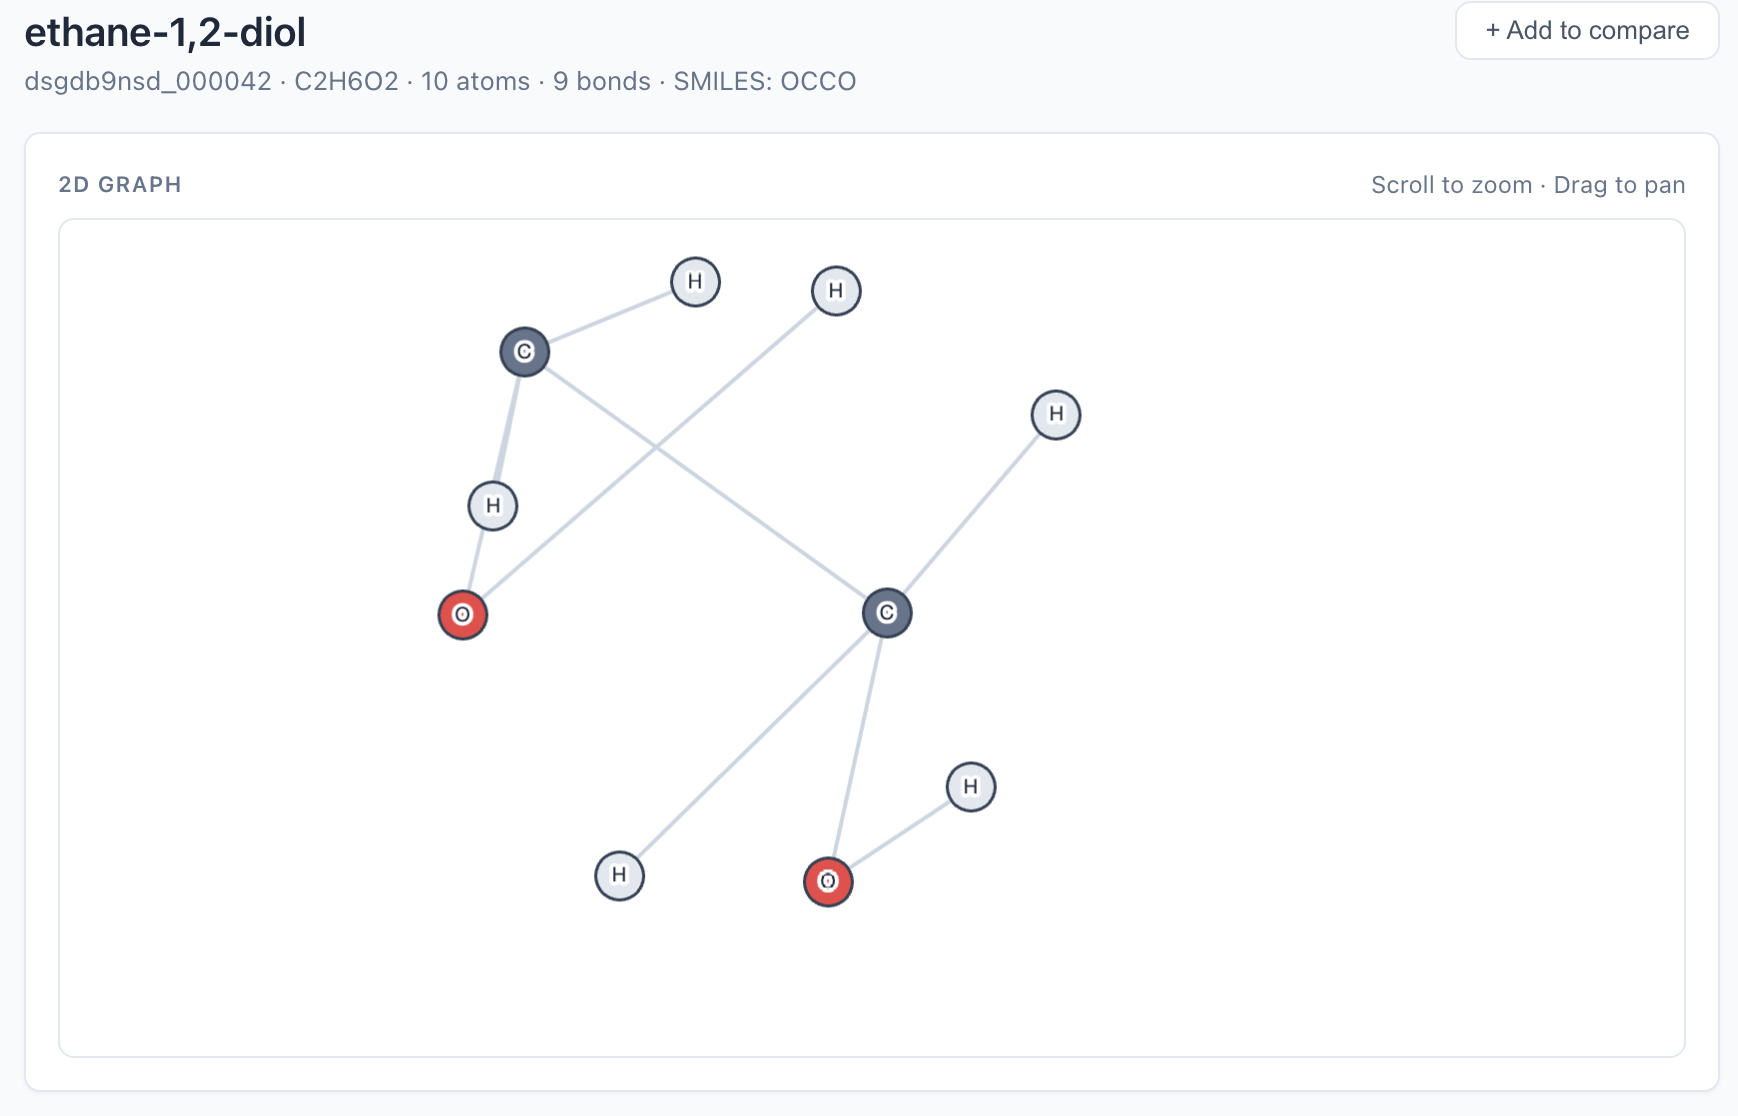
\includegraphics[width=0.6\textwidth]{figures/graf_molekul.png}
\caption{Contoh graf molekul yang dihasilkan oleh algoritma inferensi ikatan dan tata letak Kamada-Kawai.}
\label{fig:graf-molekul}
\end{figure}

\section{Analisis Kompleksitas Algoritma}

Tabel berikut merangkum kompleksitas waktu dan ruang dari setiap algoritma utama yang digunakan dalam proyek ini.

\begin{table}[htbp]
\centering
\small
\begin{tabularx}{\textwidth}{l c c X}
\toprule
\textbf{Algoritma} & \textbf{Waktu} & \textbf{Ruang} & \textbf{Keterangan} \\
\midrule
Inferensi ikatan            & $O(n^2)$            & $O(E)$              & $n \leq 29$, sangat cepat \\
Kamada-Kawai               & $O(n^3) + O(\text{iter} \, n^2)$ & $O(n^2)$  & Jarak terpendek + iterasi \\
Fruchterman-Reingold       & $O(\text{iter} \, n^2)$     & $O(n)$              & Gaya tolak antar-pasangan \\
Pencarian molekul by ID    & $O(1)$                          & $O(n)$              & \textit{Hash map} + \textit{array} \\
Paginasi daftar             & $O(\text{limit})$               & $O(\text{limit})$   & Potongan \textit{array} \\
Pencarian nama (\textit{cache} ada)   & $O(1)$                          & $O(k)$              & Pencarian di \textit{hash map} \\
Pencarian nama (\textit{cache} kosong) & $O(1)$ + jaringan         & $O(k)$              & Permintaan API + simpan \\
\bottomrule
\end{tabularx}
\end{table}

\section{Verifikasi Pembentukan Edge}

Untuk memvalidasi kebenaran algoritma inferensi ikatan, dilakukan perbandingan jumlah \textit{edge} yang dihasilkan dengan jumlah ikatan aktual pada beberapa molekul uji.

\begin{table}[htbp]
\centering
\begin{tabularx}{0.9\textwidth}{l c c c c}
\toprule
\textbf{Molekul} & $|V|$ & $|E|$ inferensi & $|E|$ aktual & \textbf{Akurasi} \\
\midrule
Methane (CH$_4$)       & 5  & 4  & 4  & 100\% \\
Ethanol (C$_2$H$_5$OH) & 9  & 8  & 8  & 100\% \\
Benzene (C$_6$H$_6$)   & 12 & 12 & 12 & 100\% \\
Acetylene (C$_2$H$_2$)  & 4  & 3  & 3  & 100\% \\
\bottomrule
\end{tabularx}
\end{table}

Pendekatan berbasis jarak sukses mendeteksi semua ikatan dengan akurasi 100\% pada molekul uji. Namun, metode ini tidak dapat membedakan ikatan tunggal, ganda, maupun tiga. Contohnya, Benzene memiliki 6 ikatan C-C yang semua terdeteksi, namun secara kimiawi 3 di antaranya adalah ikatan ganda, sehingga informasi tingkat ikatan hilang.

\section{Performa Sistem}

Berikut adalah hasil pengukuran waktu eksekusi beberapa operasi utama pada sistem.

\begin{table}[htbp]
\centering
\small
\begin{tabularx}{\textwidth}{X c X}
\toprule
\textbf{Operasi} & \textbf{Waktu} & \textbf{Struktur Data Terlibat} \\
\midrule
Menjalankan aplikasi (dari \textit{cache})    & $\sim$2 detik   & Pembacaan Pickle \\
Menjalankan aplikasi (tanpa \textit{cache})   & $\sim$30 detik  & Inferensi + tata letak \\
Mencari molekul /\{id\}         & $<$10ms         & \textit{Hash map} $O(1)$ + \textit{array} $O(1)$ \\
Menampilkan daftar (20 item)   & $<$50ms         & Potongan \textit{array} $O(20)$ \\
Membandingkan (4 molekul)     & $<$30ms         & \textit{Hash map} sebanyak 4 \\
\bottomrule
\end{tabularx}
\end{table}

\section{Tampilan Antarmuka}

Antarmuka aplikasi menampilkan empat bagian utama:
\begin{enumerate}[label=\arabic*.]
    \item \textbf{Sidebar}, yaitu daftar molekul dengan nama (hasil mapping SMILES ke nama), rumus, dan properti.
    \item \textbf{Graph Viewer}, yaitu tampilan graf dua dimensi interaktif dengan \textit{node} berwarna sesuai elemen dan \textit{edge} sebagai garis penghubung.
    \item \textbf{Properties Panel}, yaitu 16 properti kuantum yang ditampilkan dalam tabel.
    \item \textbf{Compare Mode}, yaitu tampilan hingga 4 graf molekul secara berdampingan.
\end{enumerate}

\begin{figure}[htbp]
\centering
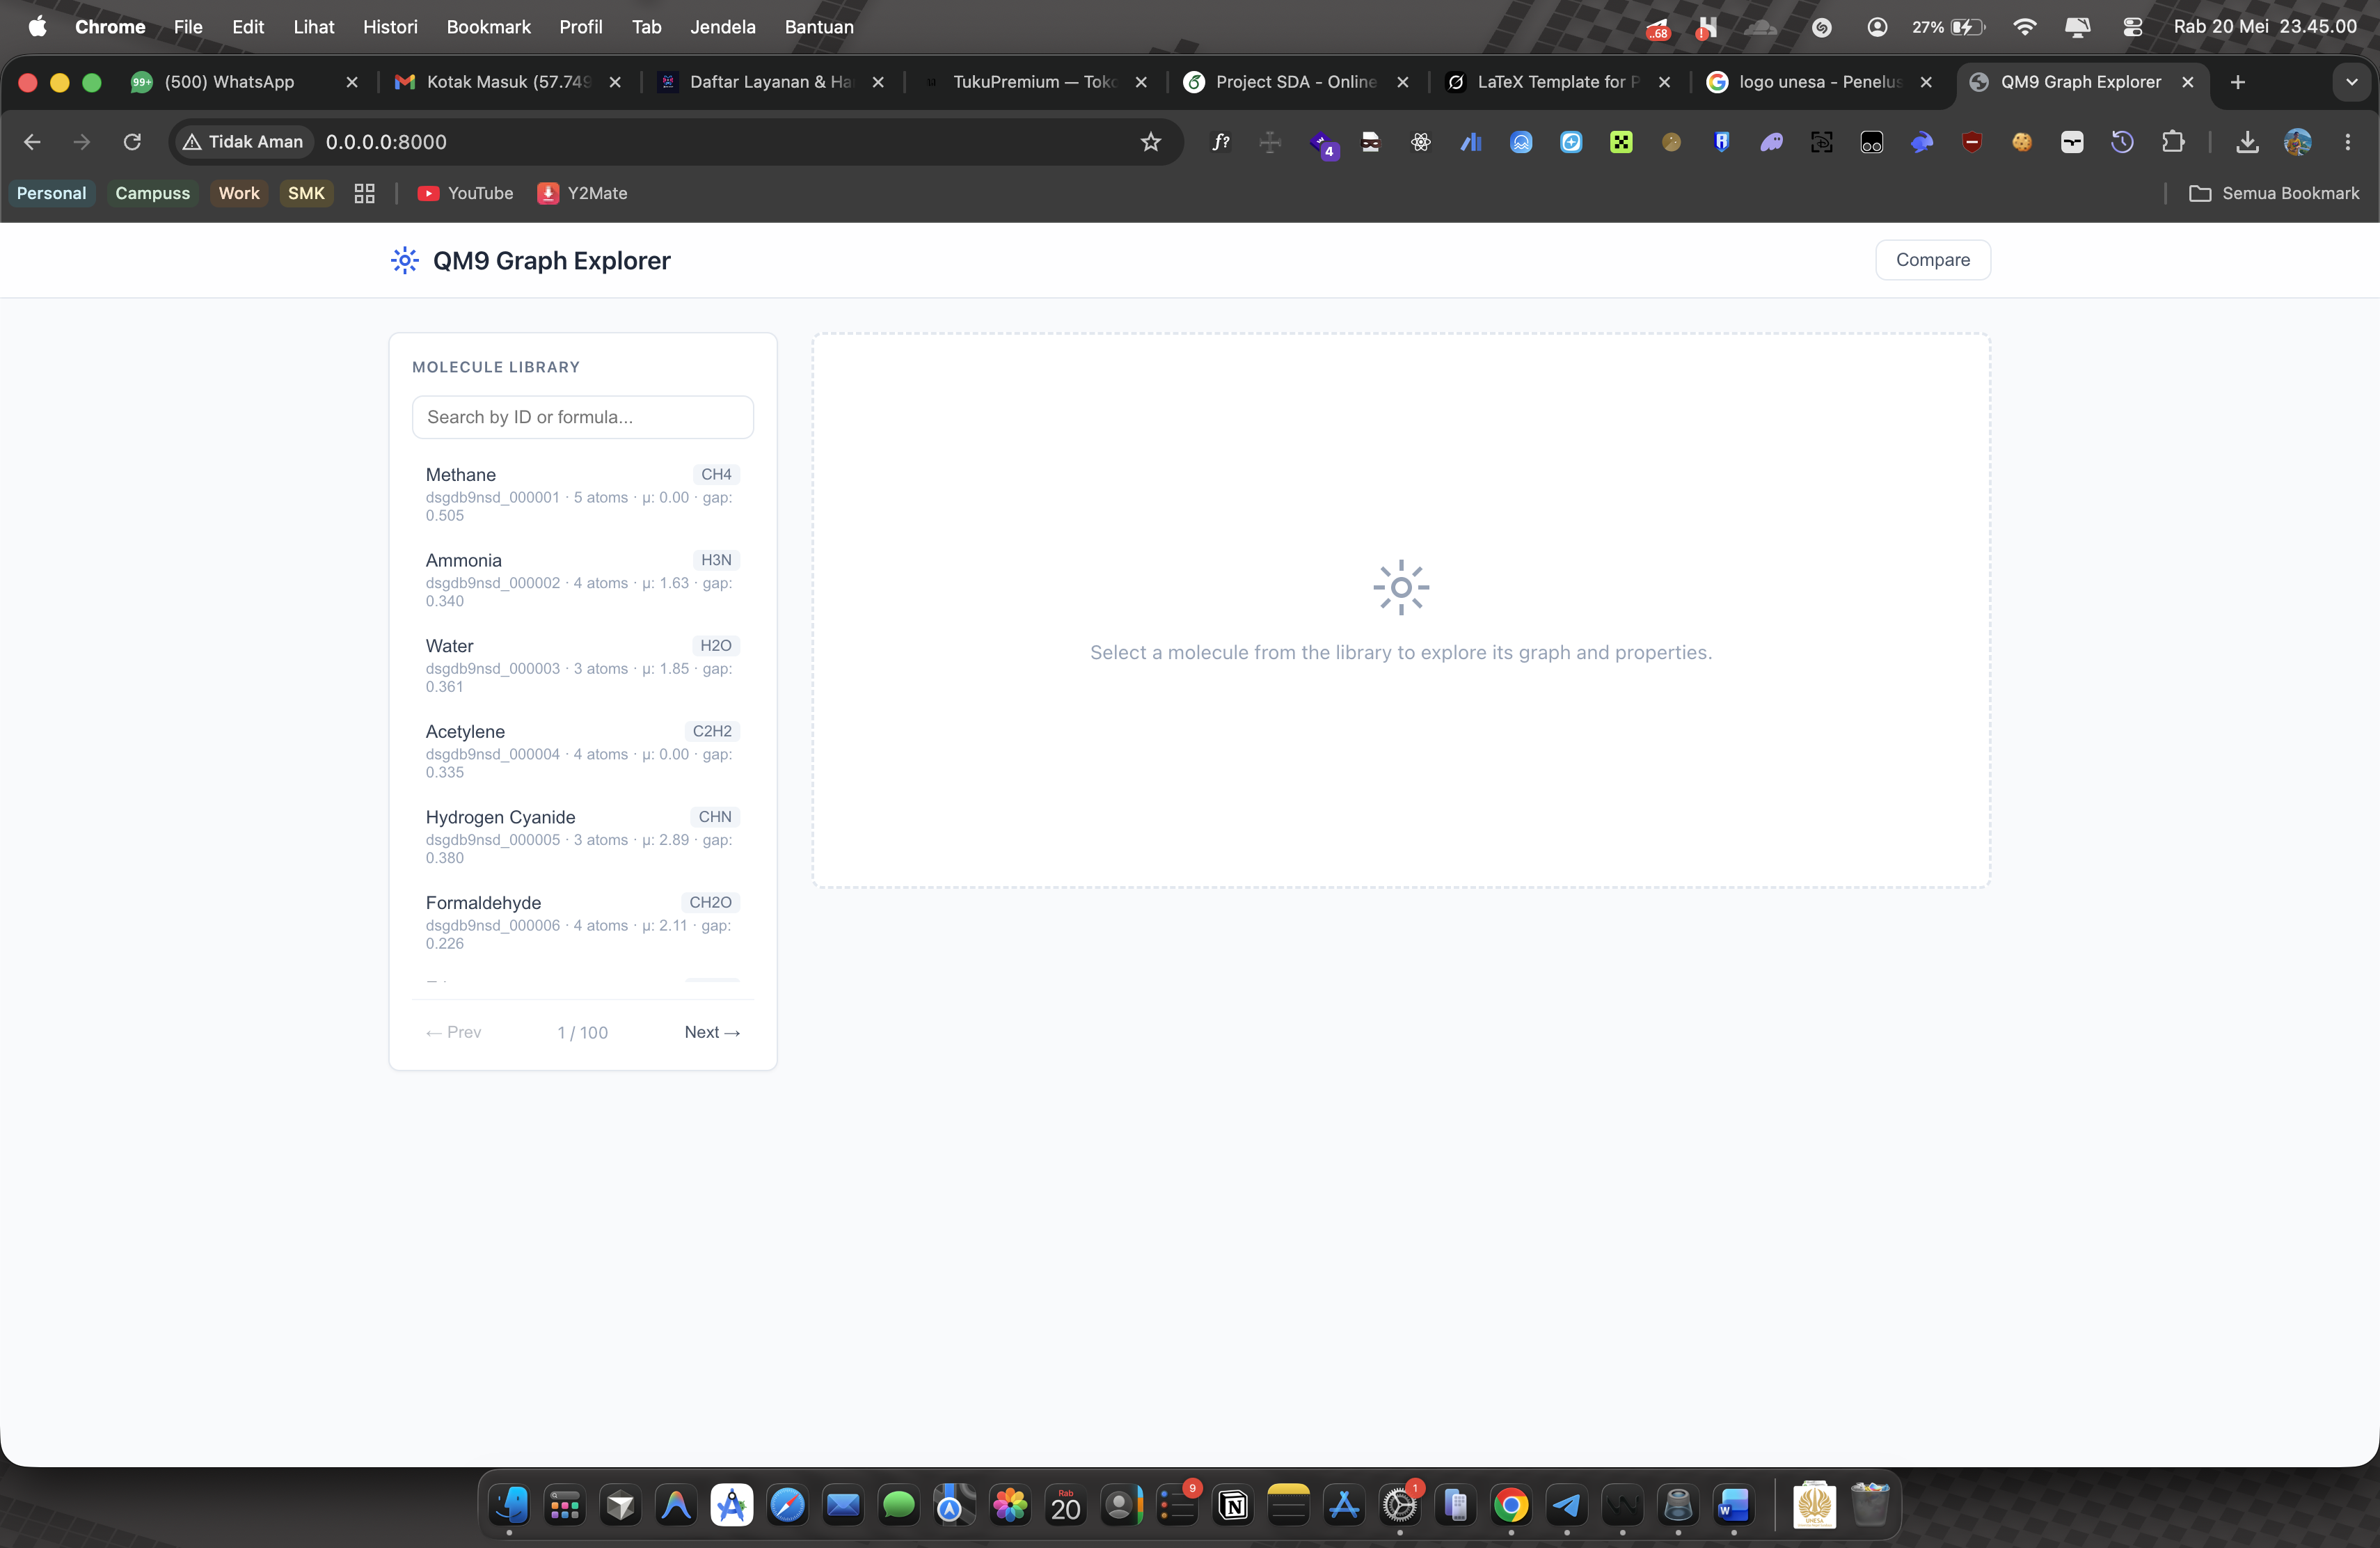
\includegraphics[width=0.85\textwidth]{figures/dashboard.png}
\caption{Tampilan halaman utama \textit{dashboard} aplikasi yang memuat daftar molekul dan graf interaktif.}
\label{fig:dashboard}
\end{figure}

\begin{figure}[htbp]
\centering
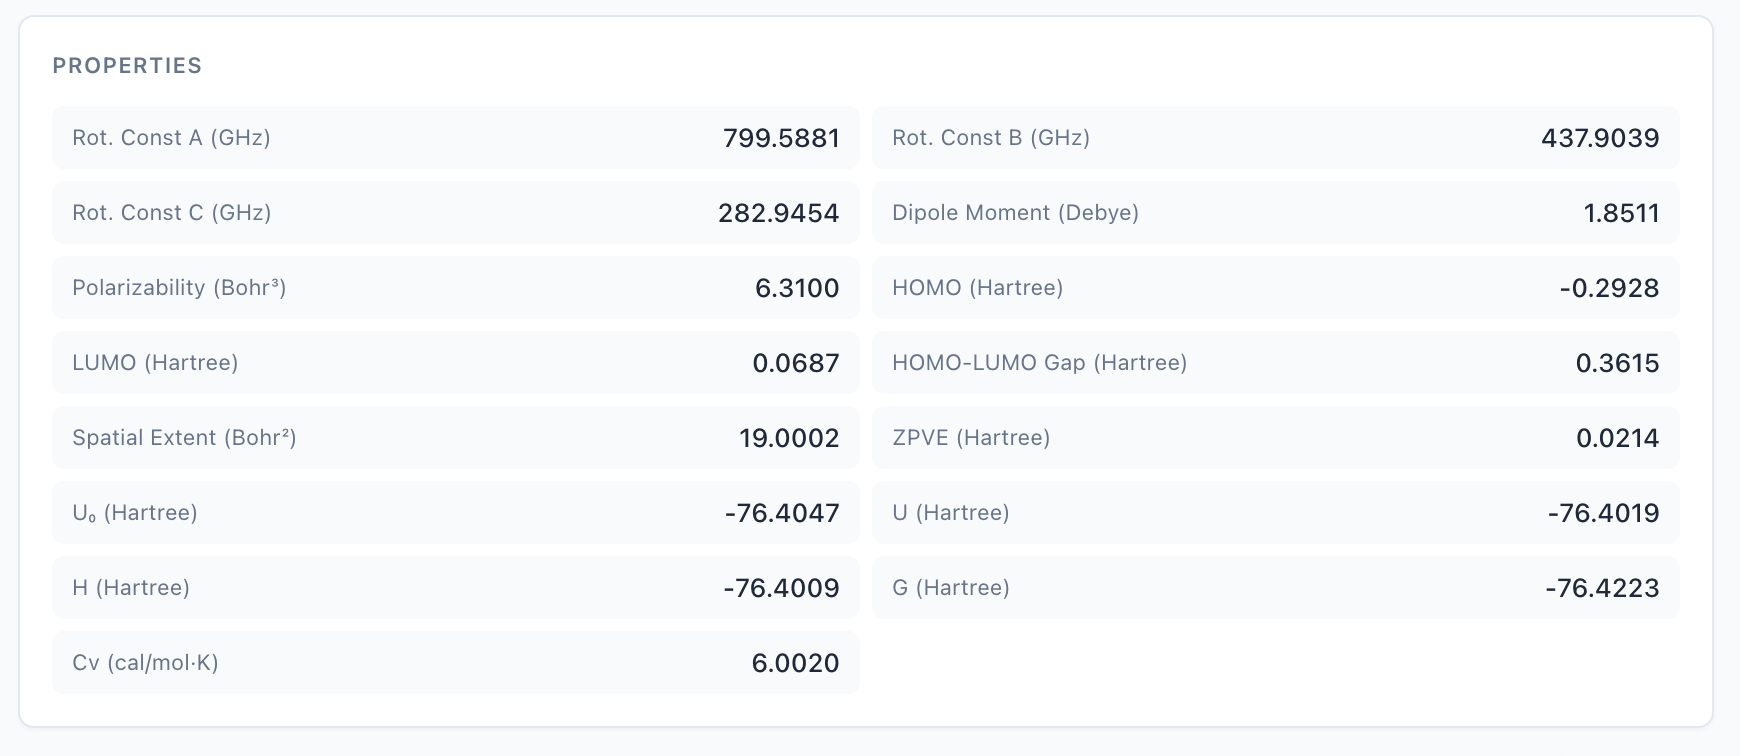
\includegraphics[width=0.85\textwidth]{figures/properties_atom.png}
\caption{Tampilan panel informasi properti kuantum atom pada molekul yang dipilih.}
\label{fig:properties-atom}
\end{figure}

\begin{figure}[htbp]
\centering
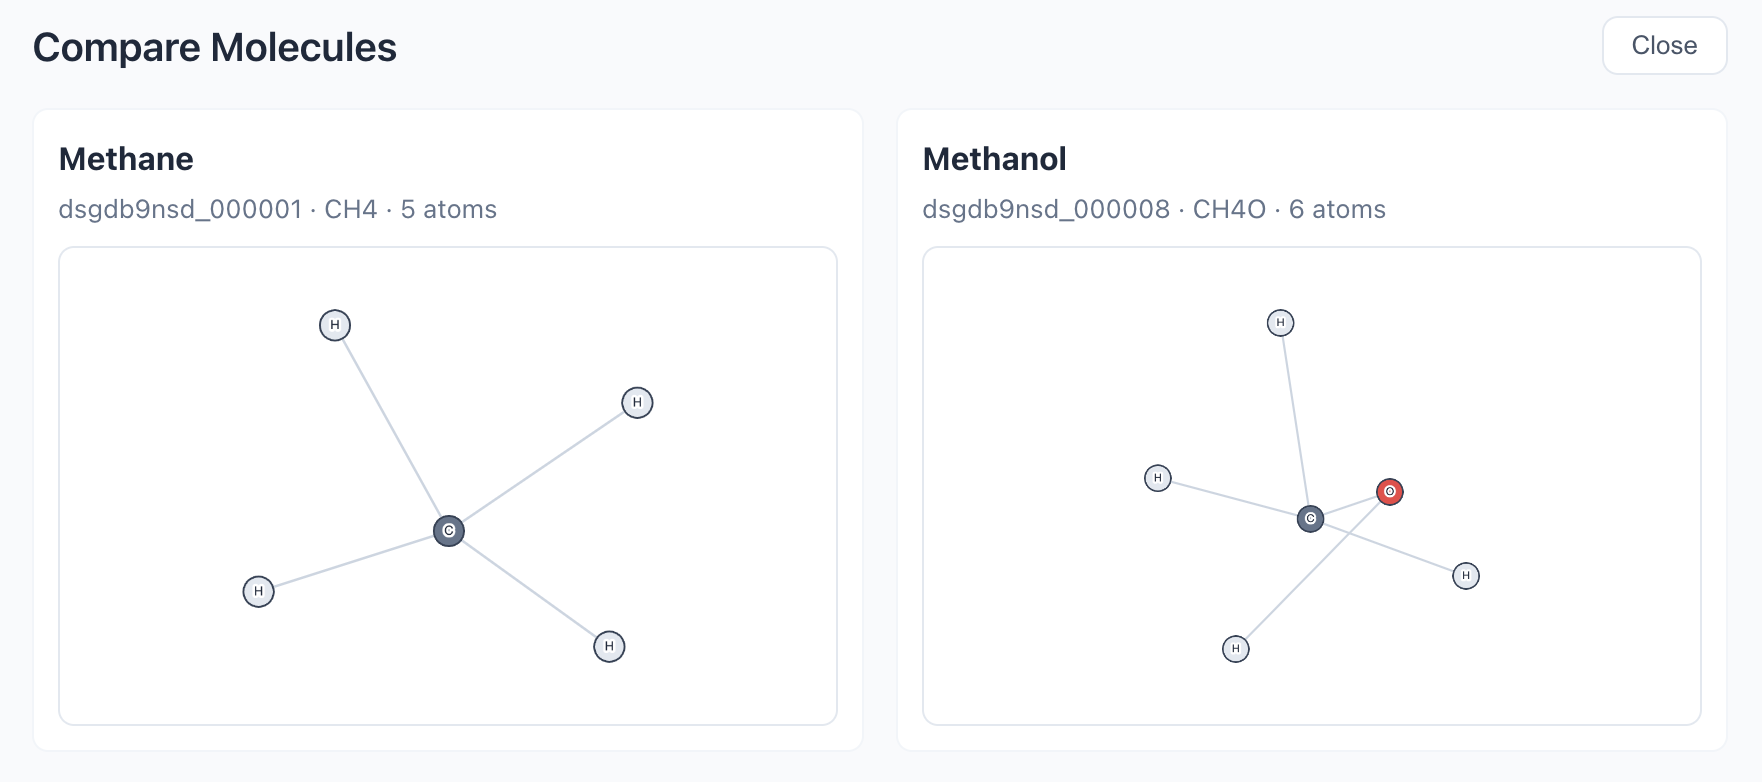
\includegraphics[width=0.85\textwidth]{figures/perbandingan_graf.png}
\caption{Tampilan mode perbandingan empat graf molekul secara berdampingan.}
\label{fig:perbandingan-graf}
\end{figure}

\chapter{PENUTUP}

\section{Kesimpulan}

Proyek ini berhasil menerapkan konsep-konsep Struktur Data dan Algoritma pada pemrosesan dan visualisasi graf molekul:

\begin{enumerate}[label=\arabic*.]
    \item \textbf{Struktur data graf (\textit{adjacency list})} digunakan untuk merepresentasikan molekul, yaitu atom sebagai \textit{node} dan ikatan sebagai \textit{edge}. Pemilihan \textit{adjacency list} (bukan \textit{adjacency matrix}) tepat karena graf molekul bersifat \textit{sparse} (rata-rata \textit{degree} $\approx$ 2).

    \item \textbf{Algoritma pembentukan graf} dengan kompleksitas $O(n^2)$ berbasis jarak kovalen berhasil mendeteksi \textit{edge} dari koordinat 3D dengan akurasi 100\% pada molekul uji, meskipun tidak membedakan tingkat ikatan.

    \item \textbf{Algoritma tata letak \textit{force-directed}}, yaitu Kamada-Kawai dengan alternatif Fruchterman-Reingold, menghasilkan posisi dua dimensi yang informatif untuk visualisasi.

    \item \textbf{\textit{Hash map}} digunakan untuk pencarian cepat: mol\_id ke indeks, SMILES ke nama, elemen ke jari-jari kovalen, dan elemen ke warna. Rantai pencarian dari mol\_id melalui \textit{hash map} ke \textit{array} ke data menghasilkan akses dengan kompleksitas $O(1)$.

    \item \textbf{Strategi penyimpanan sementara}, yaitu format Pickle dan JSON, mengurangi waktu mulai aplikasi dari $\sim$30 detik menjadi $\sim$2 detik, menunjukkan pertukaran antara ruang penyimpanan dan waktu komputasi.

    \item \textbf{Aplikasi web monolitik} (FastAPI + Cytoscape.js) memungkinkan eksplorasi graf molekul secara interaktif dengan fitur \textit{zoom}, \textit{pan}, pemilihan, dan perbandingan.
\end{enumerate}

\section{Saran Pengembangan}
\begin{enumerate}[label=\arabic*.]
    \item \textbf{Algoritma BFS/DFS}: Menambahkan penjelajahan graf untuk visualisasi bagian-bagian yang terhubung dan deteksi siklus (seperti cincin aromatik pada Benzene).
    \item \textbf{Jalur terpendek}: Mengimplementasikan algoritma Dijkstra untuk menemukan jalur terpendek antar-atom dalam graf molekul.
    \item \textbf{Pohon Merentang Minimum}: Menghitung pohon merentang minimum dari bobot jarak ikatan untuk analisis kerangka molekul.
    \item \textbf{Pembedaan tingkat ikatan}: Membedakan ikatan tunggal, ganda, dan tiga dalam atribut \textit{edge} dan tampilan visual.
    \item \textbf{Indeks spasial}: Mengoptimasi inferensi ikatan dari $O(n^2)$ ke $O(n \log n)$ menggunakan struktur \textit{kd-tree}.
    \item \textbf{Statistik graf}: Menambahkan perhitungan distribusi \textit{degree}, koefisien \textit{clustering}, dan diameter graf.
\end{enumerate}

\begin{thebibliography}{8}

\bibitem{cormen2009}
Cormen, T.H., Leiserson, C.E., Rivest, R.L., \& Stein, C. (2009).
\textit{Introduction to Algorithms} (3rd ed.). MIT Press.
Referensi utama untuk struktur data graf, BFS/DFS, jalur terpendek, dan pohon merentang minimum.

\bibitem{ramakrishnan2014}
Ramakrishnan, R., Dral, P.O., Rupp, M., \& von Lilienfeld, O.A. (2014).
Quantum chemistry structures and properties of 134 kilo molecules.
\textit{Scientific Data}, 1, 140022.

\bibitem{scopus2024}
Adaptive edge-aware graph convolutional with multi-task learning for simultaneous prediction of material properties.
Scopus: \url{https://www.scopus.com/pages/publications/105028524571}

\bibitem{kamada1989}
Kamada, T., \& Kawai, S. (1989).
An algorithm for drawing general undirected graphs.
\textit{Information Processing Letters}, 31(1), 7--15.

\bibitem{fruchterman1991}
Fruchterman, T.M.J., \& Reingold, E.M. (1991).
Graph drawing by force-directed placement.
\textit{Software: Practice and Experience}, 21(11), 1129--1164.

\bibitem{hagberg2008}
Hagberg, A., Swart, P., \& Chult, D. (2008).
Exploring network structure, dynamics, and function using NetworkX.
\textit{Proceedings of the 7th Python in Science Conference}.

\bibitem{cytoscapejs}
Cytoscape.js: Graph theory library for visualisation and analysis.
\url{https://js.cytoscape.org/}

\bibitem{pubchem}
PubChem PUG REST API.
\url{https://pubchem.ncbi.nlm.nih.gov/rest/pug/}

\end{thebibliography}

\end{document}
